\documentclass[preprint,10pt]{aastex}
%\documentclass[preprint2,12pt]{aastex}
%\documentclass[iop,onecolumn]{emulateapj}
%\usepackage{apjfonts}
\usepackage{graphicx}
\newcommand{\be}{\begin{displaymath}}
\newcommand{\ee}{\end{displaymath}}
\newcommand{\bea}{\begin{eqnarray*}}
\newcommand{\eea}{\end{eqnarray*}}
\newcommand{\pd}{\partial}


\begin{document}

% ------------------------------------------------------------------------
% New commands
%
\def\ltsima{$\; \buildrel < \over \sim \;$}
\def\lsim{\lower.5ex\hbox{\ltsima}}
\def\gtsima{$\; \buildrel > \over \sim \;$}
\def\gsim{\lower.5ex\hbox{\gtsima}}

% -------------------------------------------------------------------------
%

\bibliographystyle{apj}

\title{ Expected photon fluxes in the TESS bandpass}

\author{Peter W.\ Sullivan and Joshua N.\ Winn}

\affil{Department of Physics, and Kavli Institute for
   Astrophysics and Space Research, Massachusetts Institute of
   Technology, Cambridge, MA 02139}

\slugcomment{TESS Science Memo No.\ 2, Version 3, 2013~December~15}

\begin{abstract}

  We compute the rate of detected photons per unit collecting area
  (photons~s$^{-1}$~cm$^{-2}$) for observations within the TESS bandpass,
  for main-sequence dwarf stars of a given
  apparent magnitude and spectral type.

\end{abstract}

\section{Statement of the problem}

The precision of TESS photometry will be limited in many cases by
photon-counting noise.  Understanding the prospects for planet
detection requires accurate estimates of the number of photons that
can be detected from the target stars.

The target stars will probably be selected on the basis of apparent
magnitude and spectral type.  The apparent magnitude will be in some
broad optical bandpass, and the spectral type will be inferred from
broadband colors and whatever other information may be
available. Therefore the basic problem is to estimate the photon flux
(ph~s$^{-1}$~cm$^{-2}$) in the TESS bandpass for a star of a given
apparent magnitude and spectral type.

As described in the CSR, the target stars will be dwarfs of spectral
types F5-M5. The apparent magnitude limit will be approximately $I<12$
for the F, G, and K stars, and $I<13$ for the M stars (where $I$ is
the Cousins $I$ magnitude). The TESS bandpass ranges from
approximately 0.6--1.0~$\mu$m.

The photon flux in the TESS bandpass, denoted $\Gamma_T$, will be a function of apparent magnitude $I$ and spectral type $s$.  It can be written
\be
\Gamma_T(I,s) = \int \Gamma_\lambda(I,s)~T_\lambda~d\lambda 
= 10^{-0.4~I} \int \Gamma_\lambda(0,s)~T_\lambda~d\lambda
\ee
where $\Gamma_\lambda(I,s)$ is the photon flux density
(ph~s$^{-1}$~cm$^{-2}$~\AA$^{-1}$) of the target star, and $T_\lambda$
is
the dimensionless spectral response function of TESS. The latter equality follows
from the definition of magnitudes. To compute $\Gamma(I,s)$ we
must therefore
build reliable models for $\Gamma_\lambda(0,s)$ and $T_\lambda$,
and then perform this integral.

To set expectations it is useful to recall that Vega (A0V, $V=0.03$) has
$\Gamma_\lambda \approx 10^3$~ph~s$^{-1}$~cm$^{-2}$~\AA$^{-1}$ near
0.5~$\mu$m (Zombeck 2007, p.\ 103).  Since the TESS bandpass is
approximately 4000~\AA~wide, we expect $\Gamma_T \sim 4\times
10^6$~ph~s$^{-1}$~cm$^{-2}$ for a zero-magnitude star, or
400~ph~s$^{-1}$~cm$^{-2}$ for a 10th magnitude star.  There will be
corrections of order unity depending on the spectral energy
distributions of Vega and the target star, as well as the spectral
response functions for the $V$-band and for the TESS band.

\section{Calibrated stellar spectra}

To model the stellar photon flux densities $\Gamma_\lambda(0,s)$ we
use the spectral library of Pickles (1998), which is based on
empirical spectra gathered from various sources.  This library
includes all the spectral types needed for this study with a
wavelength coverage of 1150--10620~\AA~and a resolution of 5~\AA. The
spectra are provided as wavelength-specific flux densities $F_\lambda$
(erg~s$^{-1}$~cm$^{-2}$~\AA$^{-1}$) that are meant to have accurate spectral
shapes but are arbitrarily normalized to unity at 5556~\AA.
We must re-normalize these spectra so that they represent $I=0$ stars.

First, we normalize the A0V spectrum to have $F_\lambda = 3.44\times
10^{-9}$~erg~s$^{-1}$~cm$^{-2}$~\AA$^{-1}$ at $\lambda = 5556$~\AA, to match
the measured value for Vega (Hayes 1985).  The measurement uncertainty
is reported to be $\pm 0.05$ (1.4\%).

Next we rescale all of the other spectra so that they all have the
same $I$ magnitude as the A0V spectrum. To do so we convert
the flux densities into
photon flux densities using
\be
\Gamma_\lambda = \frac{F_\lambda}{h \nu} = \frac{\lambda F_\lambda}{hc},
\ee
and compute the integral
\be
\Gamma_I(s) = \int \Gamma_\lambda(I_{\rm arb},s) I_\lambda
\ee
where $\Gamma_\lambda(I_{\rm arb},s)$ is the arbitrarily normalized
spectrum and $I_\lambda$ is the spectral response function for the Cousins
$I$ band that is provided in Table 7 of Pickles~(1998).  We then
multiply each spectrum by a constant such that $\Gamma_I(s) =
\Gamma_I({\rm A0V})$.\footnote{Here we are assuming that magnitude
  differences specify the ratio of photon fluxes, and not energy
  fluxes, i.e., we are using a magnitude scale appropriate for
  photon-counting detectors such as CCDs.}

Finally, we multiply all of the spectra by $10^{0.4(0.035)}\approx
1.033$ because the $I$ magnitude of Vega is $0.035$ (Bessell et al.\
1998, Table A1).

\section{TESS Spectral Response}

Our model for the TESS spectral response function is the product of the CCD's quantum efficiency and the filter transmission profile. The other factors that describe the instrumental throughput have little spectral dependence, so they are factored out and considered when calculating the effective area in Section \ref{sec:aeff}. 

The quantum efficiency is provided from Lincoln Labs\footnote{{\tt QE100um\_m70.dat}} (the CCD manufacturer) for a silicon depletion depth of 100 $\mu$m. The optical filter is currently assumed to be a long-pass filter with a cut-on wavelength of 6000 $\rm \AA$. The resulting spectral response function is also plotted in Figure~\ref{fig:bandpass} along with the Sloan $griz$ bandpasses and the Cousins $I$ band (obtained from Table~7 of Pickles 1998). The instrument throughput requirements budget a transmission efficiency for the filter of 95$\%$ redward of 6000 $\rm \AA$, but that factor is considered part of the effective area in Section \ref{sec:aeff}.
%As a function of wavelength, this file tabulates the product of $25\pi$~cm$^{2}$ (the geometric area of the lens design at that time), the lens throughput, and the CCD quantum efficiency.  To obtain the dimensionless response function $T_\lambda$ we divide by $25\pi$~cm$^{2}$. 
\begin{figure}
\begin{center}
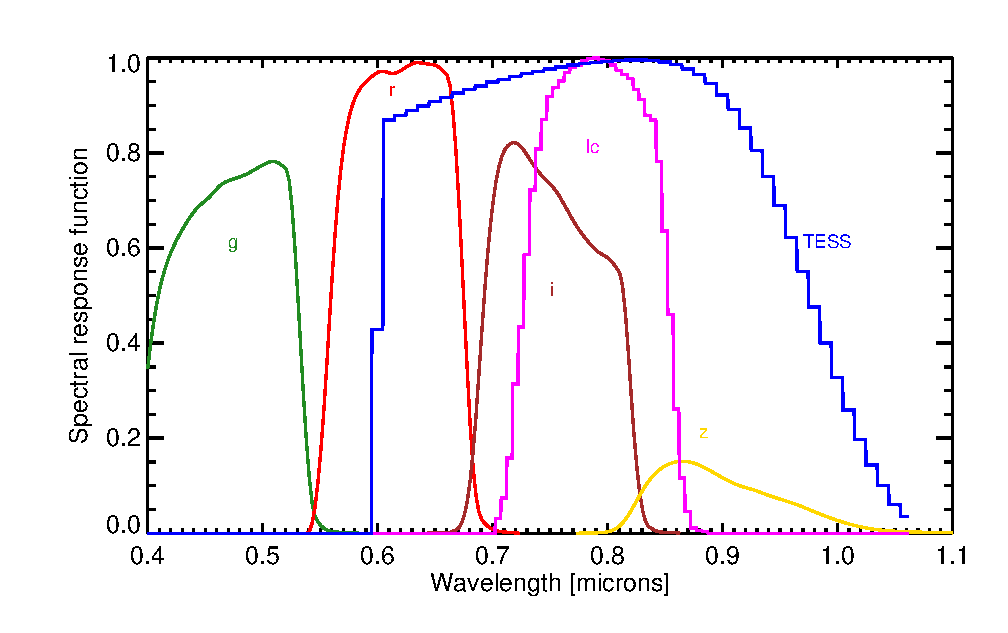
\includegraphics[width=0.7\textwidth]{bandpass.eps}
\end{center}
\caption{Spectral response functions for the TESS bandpass (blue), the Sloan $griz$ bandpasses (green, red, brown, and yellow), and Cousins $I$ (magenta). The $griz$ functions have been normalized to
a unity at the maximum of the $r$ band; their relative shapes are enveloped by the CCD quantum effieciency. The Cousins $I$ band is arbitrarily normalized to unity. The TESS function gives shows the product of the quantum efficiency and longpass filter.}
\label{fig:bandpass}
\end{figure}
 
Figures \ref{fig:pickles1} and \ref{fig:pickles2} show the photon flux
densities $\Gamma(0,s)$ for various spectral types, after performing
these calibrations. These plots also show the Sloan $gr$, Cousins $I$, and TESS bandpasses.

\begin{figure}
\begin{center}
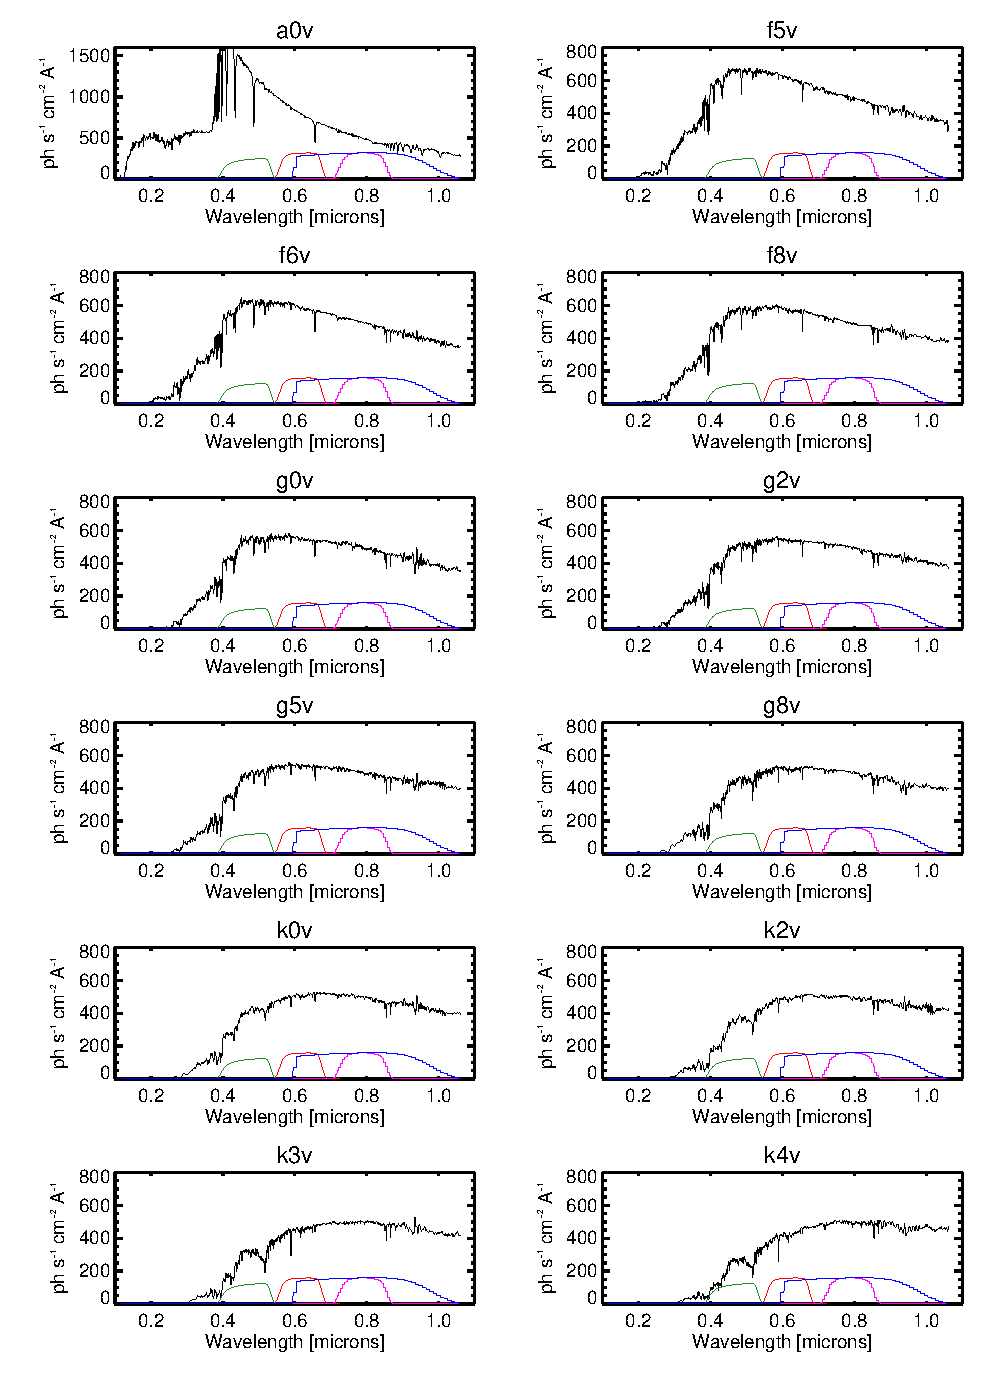
\includegraphics[width=0.8\textwidth]{pickles1.eps}
\end{center}
\caption{Photon flux densities $\Gamma(0,s)$ for stars of various
spectral types, based on the empirical library of Pickles~(1998) and
calibrated as described in the text. Spectral response functions are also shown
for Sloan $g$ (green) and $r$ (red), Cousins $I$ (magenta), 
and TESS (blue).}
\label{fig:pickles1}
\end{figure}

\begin{figure}
\begin{center}
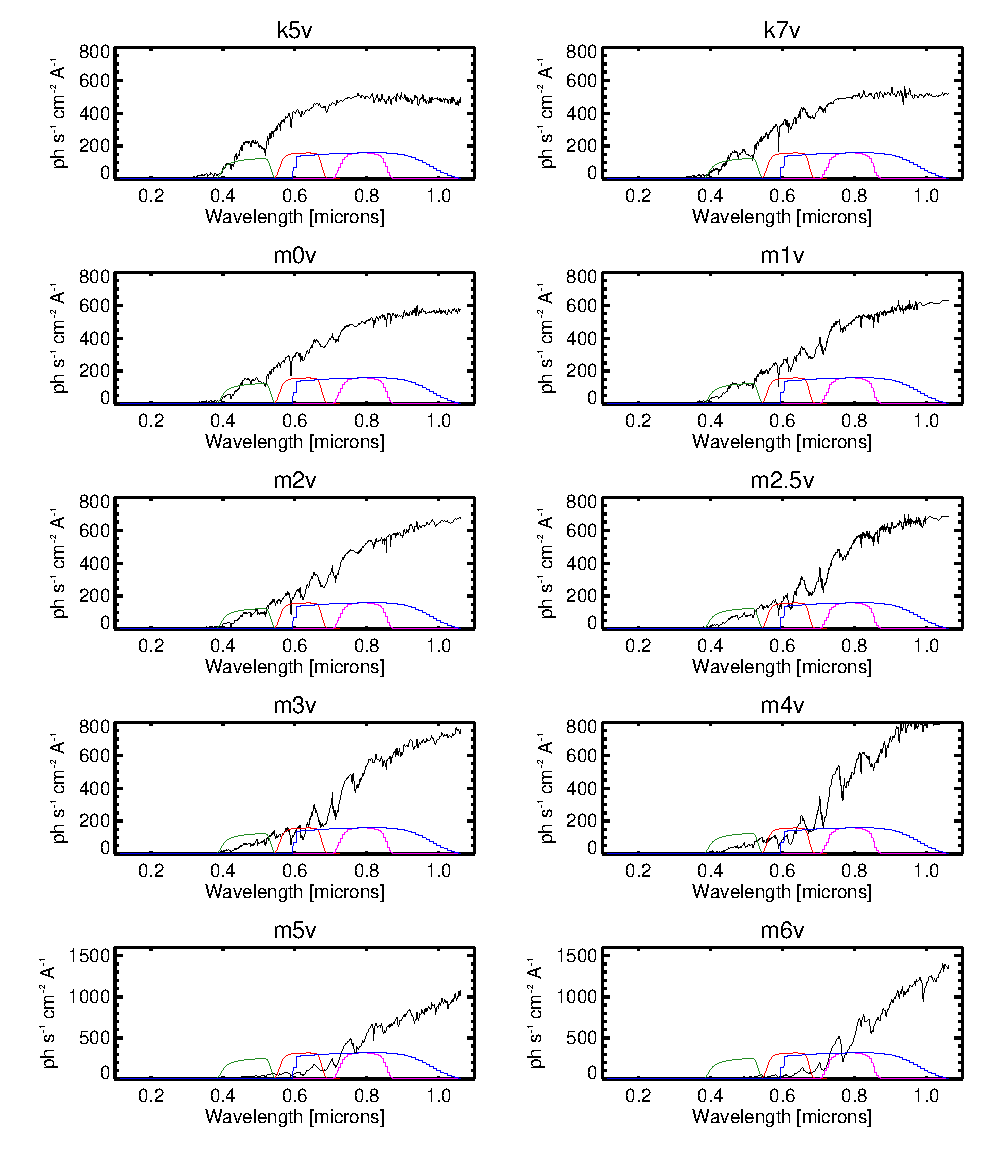
\includegraphics[width=0.8\textwidth]{pickles2.eps}
\end{center}
\caption{Photon flux densities $\Gamma(0,s)$ for stars of various
spectral types, based on the empirical library of Pickles~(1998) and
calibrated as described in the text. Spectral response functions are also shown
for Sloan $g$ (green) and $r$ (red), Cousins $I$ (magenta), 
and TESS (blue).}
\label{fig:pickles2}
\end{figure}

\section{Results}
\subsection{Photon Flux}
\label{sec:results}
The TESS photon fluxes (ph~s$^{-1}$~cm$^{-2}$) for an $I=0$ star are
computed as
\be
\Gamma_T(0,s) = \int \Gamma_\lambda(0,s)~T_\lambda~d\lambda
\ee
and shown in Figure~\ref{fig:ph_versus_teff}, as a function of 
effective temperature and spectral type\footnote{The correspondence
between $T_{\rm eff}$ and spectral type is from Pickles (1998).}. The mean is about $1.7\times
10^6$~ph~s$^{-1}$~cm$^{-2}$. This is of the order of magnitude
that was expected, based on the considerations of Section 1.
The piecewise-polynomial fit shown in Figure~\ref{fig:ph_versus_teff} is
\be
\Gamma_T(0,s)~[10^6~{\rm ph~s}^{-1}{\rm cm}^{-2}] = 1.6685, ~~ T \le 3500~{\rm K} 
\ee
\be
\Gamma_T(0,s) = 1.6685 + 
0.2145 \left( \frac{T_{\rm eff} - 3500~{\rm K}}{3500~{\rm K}} \right)
-0.0945 \left( \frac{T_{\rm eff} - 3500~{\rm K}}{3500~{\rm K}} \right)^2, ~~ T > 3500~{\rm K}
%\Gamma_T(0,s)~[10^6~{\rm ph~s}^{-1}{\rm cm}^{-2}] = 1.6301 + (2.9468\times 10^{-5}) (T_{\rm eff}~[{\rm K}] - 5000)
\ee
The results are also given in Table~1.  To obtain the TESS count rate
for a star of a given $I$ magnitude and spectral type $s$, use this
table to find $\Gamma_T(0,s)$.  Then multiply by $10^{-0.4~I}~A_{\rm
  eff}$, where $A_{\rm eff}$ is the {\it effective} collecting area
of the TESS aperture described in the next section.

\section{Effective Area}
\label{sec:aeff}
While the TESS spectral response captures the quantum efficiency and filter bandpass, 
we still must account for the optical throughput and its effect on the geometric area of the lens. The throughput factors are assumed to have little or no spectral dependence; they simply convert the geometric area to the effective area of the lens.

The geometric area is calculated simply from the entrance pupil diameter (EPD):
\be
A_{\rm geom} = \frac{\pi}{4} \left( \frac{\rm EPD} {\rm cm} \right )^2
\ee
The TESS throughput requirement budgets a filter transmission of 0.95 and an efficiency for the remaining optical elements (14 vacuum-glass interfaces and one vacuum-CCD interface) of 0.84. The effective area also departs from the geometric area as one moves off-axis by a factor of $\cos\theta$, 
where $\theta$ is the field angle (measured from the optical axis). Putting these factors together, we define the effective area as
\be
A_{\rm eff} = (0.84)(0.95) \frac{\pi}{4} \left( \frac{\rm EPD} {\rm cm} \right )^2 \cos\theta
\ee
From the CSR design, where the EPD was 9.7 cm, $A_{\rm eff}$ is $(57.6)\cos\theta$ cm$^2$. The more recent optical designs with 10.0 cm and 10.5 cm EPDs have effective areas of $(61.2)\cos\theta$ cm$^2$ and $(67.5)\cos\theta$ cm$^2$, respectively.


\begin{figure}
\begin{center}
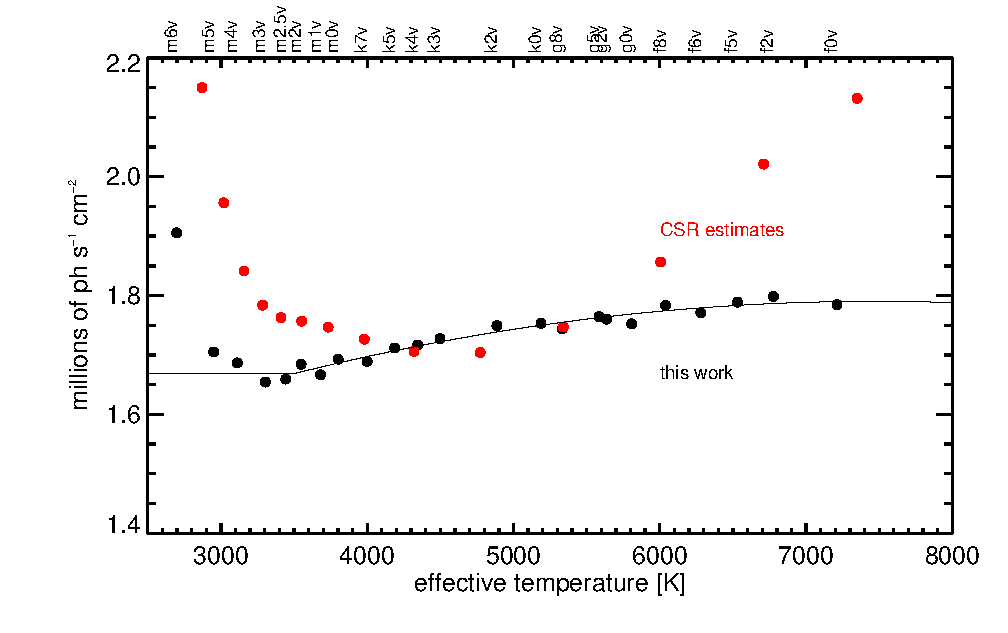
\includegraphics[width=0.7\textwidth]{ph_versus_teff.eps}
\end{center}
\caption{Photon flux in the TESS bandpass, for an $I=0$ star of
a given spectral type or effective temperature.
Black points are computed as described in this memo.
Red points are from prior calculations during the Concept Study,
based on blackbody spectra. While the photon fluxes are similar at 5000 k,
the CSR assumed an effective area of 70 cm$^2$ rather than 57.6 cm$^2$.}
\label{fig:ph_versus_teff}
\end{figure}

Finally, one should also
account for any loss of light due to the finite photometric aperture, which is covered in the exposure time calculator, 
as well as any other inefficiencies that are not captured above. For instance, antireflection coatings may lose efficiency off-axis, and the filter cut-on wavelength will vary slightly with field angle. However, these effects cannot be modeled until the design evolves further.

\section{Checks and comparisons}

The photon flux density of the A0V star is seen in
Figure~\ref{fig:pickles1} to be approximately
$10^3$~ph~s$^{-1}$~cm$^{-2}$~\AA$^{-1}$ as expected.  Visually, the
spectra in Figs.~\ref{fig:pickles1} and \ref{fig:pickles2} do appear
to be normalized to have the same $I$-band magnitude as intended.

Figure~\ref{fig:ph_versus_teff} also shows estimates for $\Gamma_T(0,s)$ that are based on prior calculations performed during the Concept Study phase of the TESS mission. These prior calculations used the same model for $T_\lambda$, but
for $\Gamma_\lambda(0,s)$ a blackbody (Planck) spectrum was used.  The shape of the Planck spectrum was determined by the effective temperature.  The normalization of the spectrum was determined by the bolometric luminosity that is associated with a dwarf star of the given effective temperature, which was taken from the theoretical stellar models of Baraffe et al.~(1998).  The $I$-band absolute magnitudes were also taken from Baraffe et al.~(1998).  These prior calculations led to photon fluxes that are generally higher than the calculations described here, by a minimum of 4\% for K stars and up to 20\% for M4-5 stars.  Given the approximate nature of both the blackbody approximation and the theoretical stellar models, this level of agreement seems reasonable.

Table F-3 of the CSR Table F-3 states that a signal-to-noise ratio of 120 will be achieved for a two-second exposure of an $I=10$ star.  Based on the results presented here, for an $I=10$ G2V star and $A_{\rm geom}=57.6$~cm$^2$, we find the photon rate to be 9800~ph~s$^{-1}$. In a two-second exposure the signal-to-noise ratio (assuming only photon-counting noise) would be 140, roughly consistent with Table F-3.

\begin{deluxetable}{lcc}

\tabletypesize{\scriptsize}
\tablecolumns{3}
\tablewidth{0pt}
\tablecaption{TESS photon fluxes at $I=0$ \label{tbl:ph_versus_teff}}

\tablehead{
\colhead{Spectral type} &
\colhead{$T_{\rm eff}$} &
\colhead{$\Gamma_T$} \\
\colhead{} & 
\colhead{[K]} &
\colhead{[$10^6$~ph~s$^{-1}$~cm$^{-2}$]}
}

\startdata
   a0v &   9549 &   1.87 \\
   f5v &   6531 &   1.79 \\
   f6v &   6280 &   1.77 \\
   f8v &   6039 &   1.78 \\
   g0v &   5807 &   1.75 \\
   g2v &   5636 &   1.76 \\
   g5v &   5584 &   1.76 \\
   g8v &   5333 &   1.74 \\
   k0v &   5187 &   1.75 \\
   k2v &   4886 &   1.75 \\
   k3v &   4497 &   1.73 \\
   k4v &   4345 &   1.72 \\
   k5v &   4187 &   1.71 \\
   k7v &   3999 &   1.69 \\
   m0v &   3801 &   1.69 \\
   m1v &   3681 &   1.67 \\
   m2v &   3548 &   1.68 \\
 m2.5v &   3443 &   1.66 \\
   m3v &   3303 &   1.65 \\
   m4v &   3111 &   1.69 \\
   m5v &   2951 &   1.71 \\
   m6v &   2697 &   1.91 \\
\enddata

\end{deluxetable}

\end{document}

\begin{thebibliography}{}

\bibitem[Baraffe et 
al.(1998)]{1998A&A...337..403B} Baraffe, I., Chabrier, G., Allard, F., \& Hauschildt, P.~H.\ 1998, \aap, 337, 403 

\bibitem[Bessell et 
al.(1998)]{1998A&A...333..231B} Bessell, M.~S., Castelli, F., \& Plez, B.\ 1998, \aap, 333, 231 

\bibitem[Hayes(1985)]{1985IAUS..111..225H} Hayes, D.~S.\ 1985, Calibration 
of Fundamental Stellar Quantities, 111, 225 

\bibitem[Pickles(1998)]{1998PASP..110..863P} Pickles, A.~J.\ 1998, \pasp, 
110, 863 

\bibitem[Zombeck(2007)]{2007hsaa.book.....Z} Zombeck, M.\ 2007, Handbook of 
Space Astronomy and Astrophysics: Third Edition (Cambridge University Press).
Available online at {\tt http://ads.harvard.edu/books/hsaa/}.


\end{thebibliography}

\end{document}
